\documentclass[12pt]{article}
\usepackage{amssymb,mathrsfs, amsmath,amsfonts,graphicx}
\usepackage{mathtools}
\usepackage{graphicx}
\usepackage{enumitem}
\usepackage{braket}
\usepackage{bbm}
\usepackage{quantikz}


\title{Problem Set 7}
\author{CSE 468}
\date{\today}
%%
%%
\newcommand{\Blank}[1][1in]{\mbox{\hskip 4pt\vrule width #1 depth 2pt}\vrule width 0pt height 2.0em}
\newcommand{\NameBlank}{\mbox{\hskip 4pt\vrule width 2.5in depth 2pt}\vrule width 0pt height 2.0em}
\newcommand{\BlankLine}{\mbox{\hskip 4pt\vrule width 5.5in depth 2pt}\vrule width 0pt height 2.0em}
%%
%% Leave at least #1 space, default to what is below
%%
\def\DefaultSpace{1in}
\newcommand{\LeaveSpace}[1][\DefaultSpace]{%
\vskip #1 plus 1fil\relax\hbox to 0pt{\hss} %
}


\begin{document}

\maketitle

\noindent Name:\NameBlank{} \newline
\noindent Student ID:\NameBlank{} \newline
\textbf{Note:} You may discuss these problems with other students, but you must write your own solutions. If you run out of space for any question, please use the additional page and clearly indicate which question you are answering.

\begin{enumerate}[font=\bfseries]

\item (20 points) Referencing the material beginning on slide 7 page 51 in 25.pdf, consider an instance of Simon with $n=10$ qubits.  

Using the formula there, how many queries must we issue classically to try to find $x$ and $y$ such that $f(x)=f(y)$ with each of the following probabilities?
\begin{description}
    \item[10\%] \Blank{}
    \item[50\%] \Blank{}
    \item[90\%] \Blank{}
    \item[99\%] \Blank{}
    \item[99.9\%] \Blank{}
\end{description}
\item(10 points) Suppose for an instance of Simon's problem we are incredibly lucky and discover in two queries that \texttt{101101} and \texttt{000111} are mapped to the same value by the oracle.  \begin{enumerate}
    \item What is the secret $s$?\Blank[1.5in]{}
    \item How many other inputs will map to the same value as do \texttt{101101} and \texttt{000111}?\Blank{}
\end{enumerate}

\item (20 points) Consider a 3-qubit system in state $\ket{\psi}$.  Suppose \[ \textbf{H}\left(\ket{\psi}\right)=\frac{\ket{001}+\ket{100}}{\sqrt{2}}\] 

What is $\ket{\psi}$? 
Hint: Hadamard is its own inverse.
\LeaveSpace{}

    \item (15 points) Consider the oracle portion of a circuit below for an $8$-bit instance of the Bernstein--Vazirani problem.  Recall the oracle computes $y=x\oplus s$ for a secret bit vector~$s$.
    
    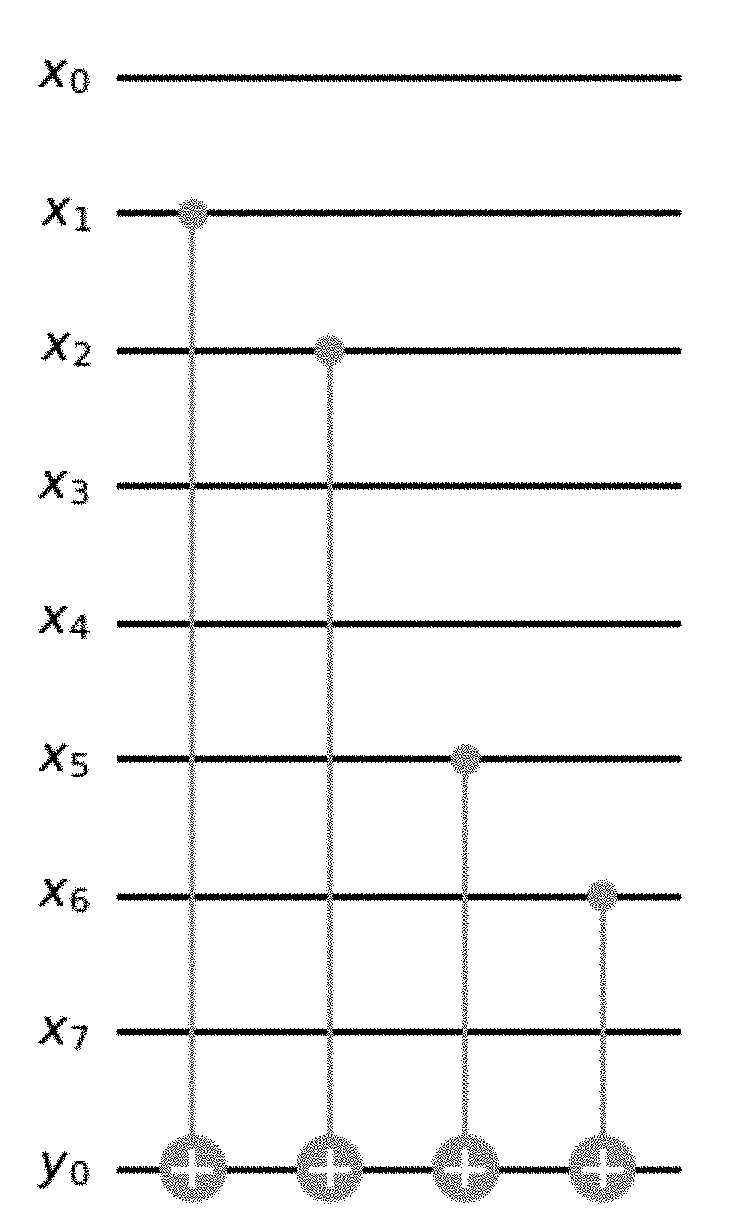
\includegraphics[scale=0.4]{ps7_assets/bv.png}
\begin{enumerate}
\item (5 points)
    What is the secret $s$ here? \Blank[2in]{}
    \item (5 points) If this oracle is used in the Deutsch--Jozsa algorithm, what possible amplitude(s) can be measured on $\ket{00000000}$?
    
    \Blank[4in]{}
    \item (5 points) What other computational basis vector(s), if any, will have non-zero amplitude for Deutsch--Jozsa if the above oracle is used?  
    
    \Blank[4in]{}
\end{enumerate}


\end{enumerate}

\end{document}